\section*{Experiment 2}
In this experiment, we explore how series and parallel combinations of \nMOS transistors behave, 
and what affect these combinations have on the channel current, \Isat, as a function of gate voltage,
\Vg. In order to accomplish this comparison, we collected data for the channel current in both ohmic 
and saturation regions of operation for a single \nMOS transistor, two transistors in parallel, and
two transistors in series, using $V_{gb} = 10mV$ and $ V_{ds} = V_{dd}$ and respectively.

\begin{figure}[H]
\centering
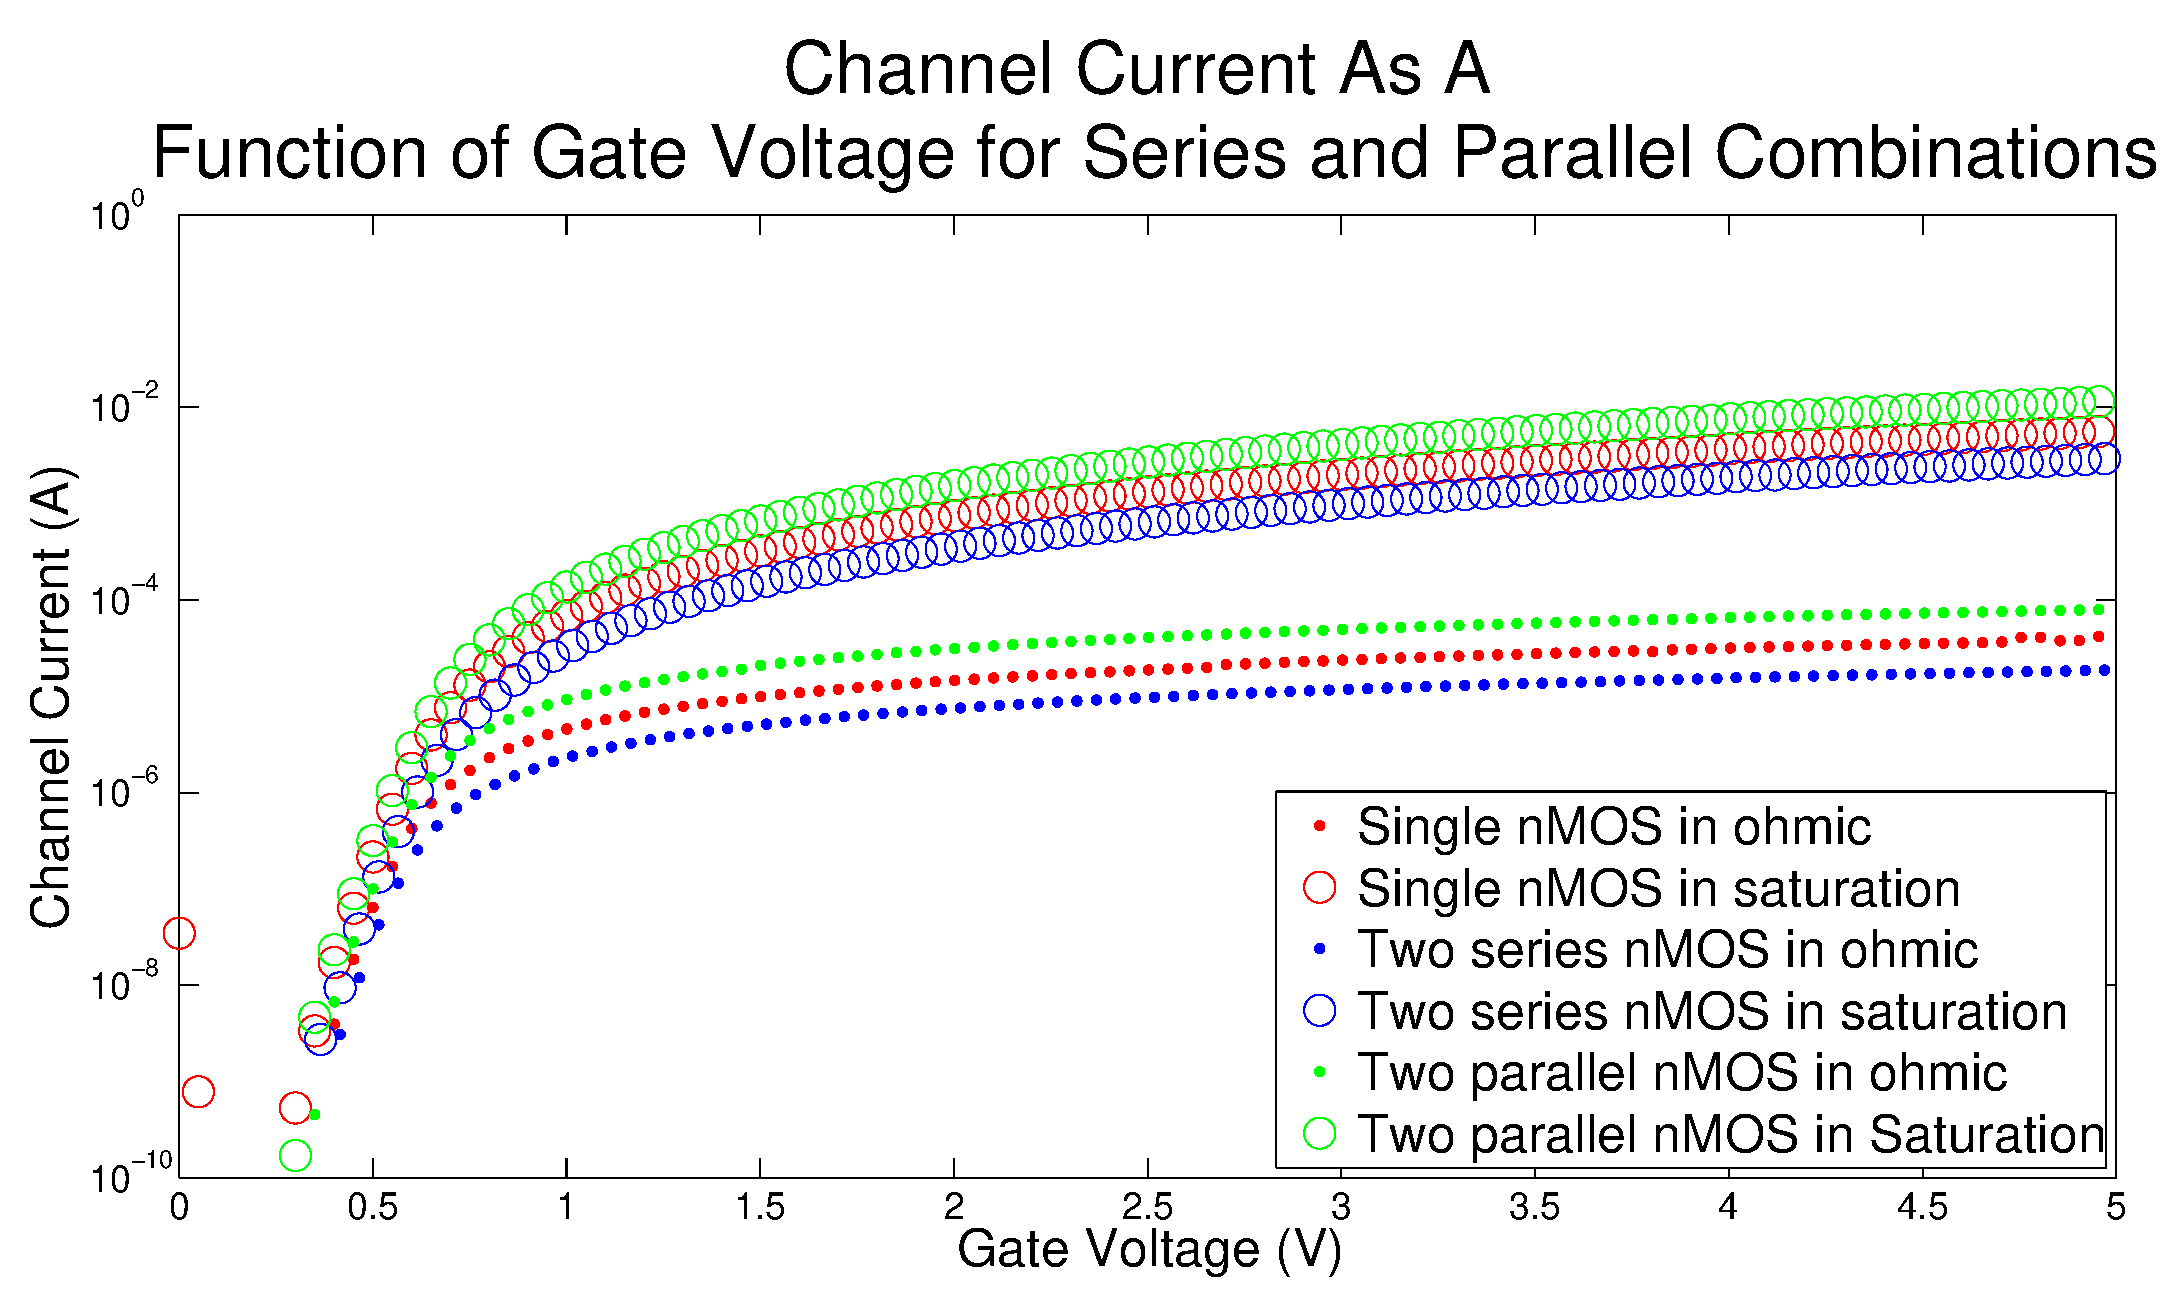
\includegraphics[width=\linewidth]{../Figures/Experiment2Currents.eps}
\caption{Note that after SMU is able to accurately measure current, after the channel current increases past roughly $10^{-8}$, the three different arrangements are separated by a constant distance in logspace, and thus appear to differ by a constant factor.}
\label{fig:nmosdia}
\end{figure}

At first glance, it seems that the channel current through the series combination is half of that through a single \nMOS with the same gate, source, drain and bulk voltages.